\documentclass{article}

\usepackage[utf8]{inputenc} 
\usepackage{outlines}
\usepackage{amsmath}
\usepackage{cleveref}
\usepackage{siunitx}
\usepackage{multirow}
\usepackage{float}

\usepackage{natbib}
\bibliographystyle{abbrvnat}

\usepackage[margin=1in]{geometry}
\parskip 1.5ex % paragraph spacing

\usepackage{graphicx}
\graphicspath{./docs/Figures/}

%external references
\usepackage{xr}
\makeatletter
\newcommand*{\addFileDependency}[1]{% argument=file name and extension
  \typeout{(#1)}
  \@addtofilelist{#1}
  \IfFileExists{#1}{}{\typeout{No file #1.}}
}
\makeatother

\newcommand*{\myexternaldocument}[1]{%
    \externaldocument{#1}%
    \addFileDependency{#1.tex}%
    \addFileDependency{#1.aux}%
}

\myexternaldocument{./docs/Maintext/SM}

\title{Variation in thermal sensitivity of ecological traits drives patterns of microbial community richness across temperature gradients}
\author{Tom Clegg, Samraat Pawar}
\date{January 2021}

\begin{document}

\maketitle

\section*{Abstract}

Variation in the thermal sensitivity of key traits is ubiquitous across the tree of life and has been demonstrated to be widespread within microbes. Whilst this variation is acknowledged to be important, relatively little work has aimed to characterise its consequences, especially on community level properties such as community dynamics, species richness and their respective thermal responses. Here using a general model of microbial community dynamics we derive analytical results which explicitly link variation in thermal sensitivity amongst microbial populations to the temperature responses of species richness. By determining the effect of variation in population-level thermal responses on the distribution of vital traits we are able to derive an expression for the temperature dependence of feasibility---the capacity of a system to support all species at equilibrium with non-zero abundance---, which we use to place an upper bound on species richness. Our results show that increasing variation in thermal sensitivity (the magnitude of species responses to temperature) results in unimodality in the species richness temperature response. We then use a newly compiled data set of microbial population growth to obtain empirical estimates of variation in microbial temperature responses which we show are both significant and sufficient to alter estimates of the species richness-temperature relationship. Finally we use numerical simulations to demonstrate the generality of our theory, showing that the relationship between variation in thermal responses and species richness hold across a range of assumptions about interaction structures within communities. Our results represent the first attempt to understand how variable population-level thermal responses scale up to affect community level properties in complex multi-species systems. They provide both, a new mechanism to explain temperature-diversity relationship in microbial communities, and a mechanistic understanding of the effect of population level trait variation on the thermal response of whole, complex microbial communities. 

\clearpage

\section*{Introduction}

The effect of temperature on biodiversity has long been a topic of interest in ecology \citep{Gaston2000}. Starting with the pioneering work of Alexander von Humboldt who in the 19th century identified temperature as a major environmental driver of plant richness along elevational gradients in the Andes (REF), many relationships between taxonomic richness and temperature have been identified across different taxa and environments with various mechanisms being suggested to explain these patterns \citep{Rohde1992,Gaston2000}. In recent years the relationship between species richness in microbial communities to temperature has become a topic of particular interest, as awareness of their importance in maintaining the key ecosystem functions increases (REF) and new sequencing technologies allow whole microbial communities to be characterised with relative ease (REF).  

Broadly the effects of temperature on microbial communities are well documented, with many studies showing how temperature affects aspects such as their structure (REF), function (REF) and patterns of diversity (REF). This temperature dependence can be explained by the dependence of these properties on individual metabolic rate which determines the capacity of individuals to grow and interact with their external environment (REF). The temperature dependence of metabolic rate is in turn determined by biochemical kinetics which are predictable, thus providing way to understand and predict the responses of emergent properties of interest \cite{Gillooly2001,Brown2004}. 

Though some consistencies in the thermal responses of microbial communities exist (REF), studies looking specifically at richness have generally found mixed responses to temperature which depend on the specific system being considered. For example, whilst REF found that soil microbe richness increased across a continental temperature gradient in North America others have found unimodal responses in tropical oceans (REF) and geothermal environments (REF), with richness peaking at intermediate temperatures. This variation in the temperature-richness relationship was further demonstrated and quantified in a meta-analysis by REF which showed that the temperature responses of microbial richness are "reliably unreliable" and that no single pattern (i.e shape or direction) dominates the temperature response in soil microbe communities. 

Unsurprisingly, the presence of such variation in the thermal responses of microbial richness has resulted in several mechanisms being suggested to explain the relationship. The metabolic theory of biodiversity (MTB) predicts that richness should increase with temperature based on the assumption of energy equivalence of populations (REF), with the log of richness following a linear relationship when plotted against the inverse of temperature (REF). This prediction is centered around the assumption of a single global temperature dependence across all taxa but has been met with limited support in microbial systems (REF). Another mechanism that has been suggested to explain the thermal response of microbial diversity is the metabolic niche hypothesis (REF), that at intermediate (non-extreme) temperatures there are more energetically viable ways to make a living, allowing greater potential diversity (REF). Although some observations of microbial richness appear to follow this predicted unimodal relationship (REF), it is by no means a universal rule. 

Whilst these studies have provided some insight into how microbial richness responds to temperature one aspect that has not been considered is the variation that exists in the thermal responses between and within different microbial taxa (REF). This variation has been highlighted by a number of studies using both meta-analyses and experimental approaches (REF), demonstrating how the temperature responses of key metabolic traits such as growth and respiration rate consistently vary between microbial taxa (REF). This variation is expected to be important in determining the responses of microbial communities to temperature through two mechanisms. Firstly, the non-linear nature of individual temperature responses means that variation in thermal response parameters across taxa will have significant effects on the distributions of metabolic traits across taxa at different temperatures \citep{Savage2004}. This in turn will affect the response of community dynamics to temperature and thus emergent properties such as richness. The potential impact of this variation becomes especially important when we consider the additional complexity of the non-linear interactions that have been shown to be important in microbial communities (REF), which may serve to amplify these effects. Secondly, variation in thermal responses will create ``thermal mismatches`` between different populations and traits which can result in altered responses to temperature at the community level (REF). This occurs as differences in thermal responses between taxa or traits result in changes to the relative trait values of populations or specific traits across temperature, resulting in shifts in system dynamics and thus emergent properties such as richness. Such effects have already been demonstrated in various ecological contexts including predator-prey (REF) and virus-host (REF) systems and will likely be important in microbial systems given the significant variation in thermal responses that  exists. 

In this paper we investigate the effects of variation in thermal sensitivity of metabolic traits in driving patterns of microbial community richness across temperature gradients. Using a general model of community dynamics we first analytically link variation in thermal sensitivity to the number of populations that can coexist within a community. In doing so we account for the effects of variation in the thermal sensitivity of key traits within communities and in the mismatches between different traits, representing the first attempt to explore the effects of this population-level variation in determining emergent community level-properties. We then use a newly-assembled data set of prokaryotic growth curves to parameterise the model to show that realistic variation in thermal sensitivity is significant and likely to be a key driver of patterns of species richness across temperature gradients in the real world. Finally, using numerical simulations of assembly of complex species-rich microbial communities, we show that our analytical results are robust and general. 

\section*{Methods} \label{Methods}

\subsection*{Theory}

Our overall approach is to first link the effects of a given distribution of key traits (i.e., growth rates and interaction strengths) to feasibility: the capacity for a community to support all populations (i.e., maintain non-zero abundance) at equilibrium  \citep{Grilli2017,Dougoud2018}. Feasibility is a necessary condition for stable population coexistence, and by deriving an expression for feasibility we are able to determine the maximum richness a system will be able to support given their specific trait values. 

\subsubsection*{Community Model}
In order to quantify the effects of temperature on feasibility and richness, we use the generalised Lotka-Volterra model (GLV) of an $N$ species community, with the growth of the $i$th species given by
\begin{equation} \label{EQ:GLVM}
  \frac{1}{x_i} \frac{dx_i}{dt} = r_i(T) - \sum^N_{j = 0} a_{ij}(T) x_j, 
\end{equation}
where $x_i$ is its biomass density (abundance) ($\text{mass} \cdot \text{volume}^{-1}$), $r_i(T)$ it's intrinsic growth rate determining the rate at which new biomass is produced ($\text{time}^{-1}$), $a_{ij}(T)$ is the effect of interactions with the $j$th species' population (with $a_{ii(T)}$ representing the strength of of intraspecific interactions; $\text{volume} \cdot \text{mass}^{-1} \cdot \text{time}^{-1}$). All parameters are functions of temperature ($T$), the forms of which will be addressed later. We have arbitrarily chosen to consider a three dimensional environment here, but our results are independent of this assumption as long as microbial species' abundances and interactions can be meaningfully quantified in 2D or 1D environments.  

\subsubsection*{Feasibility and Species Richness} \label{SEC:Feas_SP_rich}

We next derive an expression to determine the feasibility of a community in terms of the parameters in \cref{EQ:GLVM} and species richness. Though we consider only feasibility here, previous work has shown that in GLV systems feasible fixed points are almost always stable (REF). Thus, if we want to determine how many populations will be able to persist in a given community it is sufficient to show that the maximum number of species a community may have and remain feasible, therefore ensuring that it is dynamically stable and that populations within will thus be able to persist. 

In order to determine the feasibility of a community we need to first derive an expression for equilibrium biomass, $x^*_i$. Though it is not possible to derive an exact analytical solution for the GLV (\cref{EQ:GLVM}), we use a mean-field approximation (see \cref{SI_Sec:Meanfield} for full derivation;  \citet{Wilson2003,Wilson2004}), which allows us to derive an expression for equilibrium biomass in terms of the average effect of interactions ($\bar{a}$) across the community as: 
\begin{equation}\label{EQ:MF_equi}
  x^*_i \approx K_i(T) -  \bar{K}(T)  \frac{ (N-1)\bar{a}(T)}{1 + (N-1)\bar{a}(T)}. 
\end{equation}
Here, $K_i = \frac{r_i(T)}{a_{ii}(T)}$ is the $i$th species' carrying capacity (the biomass this population would reach if grown in isolation, obtained by solving \cref{EQ:GLVM} with no interactions), $N$ is species richness, and $\bar{a}(T)$ and $\bar{K}(T)$ are the average pairwise, interspecific interaction strength and carrying capacity respectively. \Cref{EQ:MF_equi} provides an intuitive expression for equilibrium biomasses; a population will reach the biomass that it would in isolation (first term, $K_i(T)$) minus the effects of any interspecific interactions (second term). The strength of these interspecific interaction effects is determined by the average carrying capacity of all other species ($\bar{K}(T)$) and a saturating function of the interspecies interaction strength experienced by the focal species, $(N-1)\bar{a}(T)$. If interactions are overall competitive (i.e., $\bar{a}(T) > 0$) then equilibrium biomass will be reduced relative to the individual carrying capacities, and if they are facilitatory (i.e., cooperative or mutualistic; $ \bar{a}(T) < 0$), it will increase. This approximation (\cref{EQ:MF_equi}) relies on the assumption that the system is large (i.e., $N$ is large) and that no individual pairwise interaction dominates the dynamics, but we show below that it works well for small community sizes as long as the assumption of non-dominance of any interaction holds. We also set all intraspecific interactions to $1$ to allow easier interpretation of the analytic results, though the mean-field approximation has been shown to be valid when allowing intraspecific interactions to deviate from 1 \citep{Wilson2004}. 

Next, we use \Cref{EQ:MF_equi} to derive an expression for community feasibility in terms of the population-level traits (i.e., the $r(T)$'s and $a(T)$'s) which will then be used to determine the upper bound on species richness $N$. An ecosystem is feasible if all species have non-zero equilibrium biomasses (i.e., $x_i^* > 0 $), a condition that can be expressed as:
\begin{align} \label{EQ:Feas_sp}
  \kappa_i(T) > \frac{(N-1)\bar{a}(T)}{1 + (N-1)\bar{a}(T)} \quad \text{for all} \quad i = 1 \ldots N.
\end{align}
Here, $\kappa_i = \frac{K_i(T)}{\bar{K}(T)}$ is the relative carrying capacity of the $i$th species. \Cref{EQ:Feas_sp} shows that an ecosystem is feasible as long as the the effects of interspecific interactions on each population (RHS) do not outweigh it's mean normalised carrying capacity (LHS). If interactions are competitive ($\bar{a}(T) > 0$) and strong, the inequality will not hold, extinctions will occur and the system will be unfeasible. If interactions are on average facilitatory ($\bar{a}(T) < 0$) then the LHS will always be negative and the inequality will hold as by definition $\kappa > 0$. This means that in the case where facilitative interactions dominate, feasibility is guaranteed and we cannot place an upper bound on richness. As such we focus the rest of our analytical work determining the richness-temperature relationship on the case where competitive interactions dominate ($\bar{a} > 0$), though we show later that the general insight provided by this approach applies to a range of interaction structures using numerical simulations. 

Using \cref{EQ:Feas_sp} we next derive an expression for $P_{feas}$, the probability that a community is feasible given the distribution of species trait values ($\kappa$'s and $a$'s) and number of species ($N$) in the system. To do so we take \cref{EQ:Feas_sp} and consider $\kappa$ and $a$ as random variables, each describing the distribution of the respective traits across the populations in the community (denoted by the loss of subscript). This allows us to consider $\kappa$'s cumulative density function (CDF), i.e., the probability that it is less than or equal to some value: $F_{\kappa}(x,T) = P(\kappa \leq x)$. As the condition for feasibility states that $\kappa$ must be greater than the effect of interactions we can use this CDF and the condition in \cref{EQ:Feas_sp} to express $P_{feas}$ as
\begin{equation} \label{EQ:P_feas}
    P_{feas} = P \left( \kappa(T) > \frac{(N-1)\bar{a}(T)}{1 + (N-1)\bar{a}(T)}  \right)^N = 
    \left[1 - F_{\kappa}\left(\frac{(N-1)\bar{a}(T)}{1 + (N-1)\bar{a}(T)},T \right)\right]^N,
\end{equation}
giving the probability of feasibility of an ecosystem as a function of species' traits. Note that the expression is raised to the $N^\text{th}$ power because the term in the brackets must hold for all $N$ populations in a community for it to be feasible. \Cref{EQ:P_feas} makes explicit the effect of species richness $N$ on the probability of feasibility of a community, showing how $P_{feas}$ will decline with increasing $N$ through two mechanisms. Firstly, it alters the strength of interactions experienced by individual populations via the $(N-1) \bar{a}(T)$ term. A higher species richness means that the strength of interactions will be greater and if interactions are on average competitive ($\bar{a}(T) > 0$) this will reduce the chance the condition in \cref{EQ:P_feas} is met, reducing the probability of feasibility. Secondly, the probability of feasibility will fall as the number of species increases as it becomes less likely that all $N$ species meet the criteria in \cref{EQ:Feas_sp} as represented by the $N\text{th}$ power term in \cref{EQ:P_feas}. 

Importantly, this decline in $P_{feas}$ with increasing richness places an upper bound on species richness given a certain distribution of $\kappa$ and $a$ values within a community. If a system is too large then we expect that it will have a low probability of feasibility and thus be likely to experience population extinctions until the probability of feasibility becomes larger and extinctions become unlikely. Although ideally we would use \cref{EQ:P_feas} to determine this bound explicitly by solving for $N$ this is not possible for most distributions of $\kappa$ due to the complexity of their CDFs. We therefore use a numerical approach to determine the exact value of this upper bound on $N$ (see \cref{SI_Sec:TPC_dist}). It is important to note that this does not preclude insights into the effects of variation in thermal sensitivity, which we now address. 

\subsubsection*{Thermal responses of traits} \label{SEC:Temperature}
Having defined the relationship between species richness and the distribution of species' traits across the community, we now turn to the effect of temperature. Broadly, our approach here is to consider how the distributions of the relevant species traits across populations change with temperature and thus $P_{feas}$, and ultimately (the upper bound on) $N$. We derive expressions for these trait distributions in terms of the distributions of their thermal sensitivity. This allows us to quantify the effect of variation in thermal sensitivity between species' populations as well as traits on the temperature-species richness relationship. We use the Boltzmann-Arrhenius equation to represent the temperature dependence of $\kappa$ and $a$ (Savage 2004 am nat):
\begin{equation} \label{EQ:Boltzmann}
    B(T) = B_0 e^{-\frac{E}{k} \left(\frac{1}{kT} - \frac{1}{k T_{ref} }\right)}.
\end{equation}
Here, $B(T)$ is the relevant trait value,  $T$ is temperature in Kelvin, $B_0$ is the normalisation constant, i.e., the trait value at some reference temperature ($T_{ref}$, also in Kelvin), $E$ (eV) is the thermal sensitivity which determines the change in trait value to a unit change of $\frac{1}{kT}$, and $k$ is the Boltzmann constant. Although empirically-measured thermal performance curves of single individuals or species are generally unimodal, the Boltzmann-Arrhenius equation adequately captures the the rising portion (before the temperature peak) of these curves, which is also the temperature range within which individuals and populations typically operate (or experience) (the ``Operational Temperature Range'', or OTR; \cite{Dell2011}). Thus focusing on the Boltzmann-Arrhenius portion of thermal performance curves is relevant to the dynamics of real ecosystems, and also, conveniently, affords us analytic tractability.

Applying \cref{EQ:Boltzmann} allows us to characterise the distributions of parameters across species populations at different temperatures in terms of the distributions of the underlying parameters $B_0$ and $E$. Assuming that the trait value, $B(T)$, follows a log-normal distribution across the community we let $\log(B_0)$ and $E$ both follow normal distributions, allowing us to obtain an explicit expression for the temperature dependent distribution of $B(T)$ (see \cref{SI_Sec:TPC_dist}):
\begin{align} \label{EQ:Boltz_dist}
    \log(B(T)) \sim \mathcal{N}\left(\mu_{B}(T) , \sigma_{B}^2(T) \right) 
    \quad \text{where} \quad
    \begin{array}{cc}
        \mu_B(T) &= \mu_{B_0} - \mu_{E} \left(\frac{1}{kT} - \frac{1}{k T_{ref} }\right)  \\
        \sigma_{B}(T)^2 &= \sigma_{B_0}^2 + \sigma_{E}^2 \left(\frac{1}{kT} - \frac{1}{k T_{ref} }\right)^2 .
    \end{array}
\end{align}
Here, $\log(B_0)$ and $E$ are both normally distributed, with $\mu$ and $\sigma$ denoting their mean and standard deviations respectively. \Cref{EQ:Boltz_dist} makes explicit the effect of the distribution of thermal response parameters on the distribution of $B(T)$, showing how both $\mu_{B}(T)$ and $\sigma_{B}T$ are functions of temperature. In both cases the parameters determining the distribution of $B_0$ act as constants, with the strength and nature of the temperature response being solely determined by the distribution of $E$ values. The average thermal sensitivity $\mu_E$ determines the strength of the relationship thermal response of $\mu_B(T)$ as a linear function whilst $\sigma_E$ determines the thermal response of $\sigma_{B}(T)$ as a quadratic. It is important to note that as $B(T)$ has a log-normal distribution its moments are determined by both $\mu_B(T)$ and $\sigma_B(T)$ and thus both temperature dependent factors (the linear and quadratic parts) will determine it's shape in linear scale.

Applying \cref{EQ:Boltz_dist} to the distributions of $\kappa$ and $\bar{a}$ we obtain the expressions
\begin{align} 
        \log(\kappa(T)) &\sim \mathcal{N}\left( -\frac{\sigma_{K}^2(T)}{2} , \sigma_{K}^2(T) \right) \quad \text{and} \label{EQ:Trait_distributions_K} \\ \nonumber \\
        \bar{a}(T) &= \exp \left(\mu_a(T) + \frac{\sigma_a^2(T))}{2} \right) \label{EQ:Trait_distributions_a},
\end{align}
which show how the temperature responses of $\kappa$ and $\bar{a}$ are determined by their respective thermal response parameter distributions. \Cref{EQ:Trait_distributions_K,EQ:Trait_distributions_a} show that distribution of $\kappa$ is is independent of the mean $\mu_{K}(T)$, being fully determined by the variance term $\sigma_{K}^2(T)$ whilst $\bar{a}$ is determined by both the average $\mu_a(T)$ and variance $\sigma_a^2(T)$ terms. This means that moments defining the distribution of $\kappa$ will include only the quadratic temperature terms, the strength of which is determined by the variation in thermal sensitivity $\sigma_{E_{\kappa}}$. $\bar{a}$ will also include the linear temperature term the strength of which is determined by the average thermal sensitivity, $\mu_{E_a}$. 

Combining \cref{EQ:Trait_distributions_K,EQ:Trait_distributions_a} with the equation defining $P_{feas}$, \cref{EQ:P_feas}, provides important insights into the effect of the distribution of species' trait-level thermal response parameters on the thermal response of community-level species richness. The overall direction and magnitude of the richness-temperature relationship will be determined by the average thermal sensitivity of interactions $\mu_{E_a}$ as the only linear temperature term, with richness following the inverse temperature dependence of interaction strength (as stronger competitive interactions result in lower richness as per \cref{EQ:P_feas}). The variation in thermal sensitivity, $\sigma_{E_a}$ and $\sigma_{E_{\kappa}}$ will determine the relative strength of the quadratic term in the richness temperature relationship and only when variation is large enough will it be large enough to introduce curvature in the richness temperature response. The average thermal sensitivity of carrying capacity will not affect the species richness relationship as feasibility (and thus the upper bound on richness) is defined in terms of relative carrying capacity and is independent of it's mean value. 

\subsection*{Calculating the thermal response curves of Species Richness} \label{SEC:Temp_SP_num}

In order to obtain quantitative predictions of the effect of temperature on species richness from the analytic expressions above, we substitute \cref{EQ:Trait_distributions_K,,EQ:Trait_distributions_a} into the expression for $P_{feas}$ (\cref{EQ:P_feas}), and solve for $N$. Whilst ideally this would be done analytically, the complexity of the CDF for the distribution of $\kappa$ prevents this approach and we instead solve for $N$ numerically. To this end, we set a lower threshold value of probability of feasibility, $\theta = 0.5$, as well as values for the parameters controlling the distributions of the thermal responses for both $a$ and $\kappa$. We then calculate the probability of feasibly across a range of $N$ values ($1 - 1000$ here) using \cref{EQ:P_feas} to find the maximum species richness value that has a probability of feasibility greater than the threshold $\theta$ we set. Repeating this procedure at different temperatures gives the full temperature richness curve for any given set of parameters. We calculated such species richness - Temperature curves for different combinations of means and variances of thermal sensitivity of $K$ and $a$. Holding either $\kappa$ or $a$'s distributions constant, we calculated species richness curves in a fully factorial manner setting ($\mu_{E} \in [-0.65, 0.0, 0.65]$ and $\sigma_{E} \in [0.0, 0.5, 1.0]$). We did not vary the average thermal sensitivity of $K$ as \cref{EQ:Trait_distributions_K} shows the realised distribution of $\kappa$ is independent of the average value. We also fix the distribution of normalisation constants, using the empirical distributions discussed below for $\kappa$ and setting $\mu_{a_0} = -2$ and $\sigma_{a_0} = 0.5$.

\subsection*{Data} \label{SEC:DATA}

To explore the relevance of variation in thermal sensitivity on species richness, we compiled a new data set of prokaryotic population growth curves at different temperatures to obtain realistic estimates of the distributions of thermal response parameters across species. We then use this empirical distribution to parameterise our analytical expression for feasibility and calculate the resultant species richness temperature response to explore the effects of  realistic levels of variation in thermal responses. 

Our dataset was constructed by digitising 875 individual growth curves (i.e., measurements of biomass or population size over time) representing 224 species/media combinations for which we have measurements over multiple temperatures. These growth curves were spread across unique 105 strains from 21 separate studies. We fit the logistic growth model to each of these individual growth curves using non-linear least squares, giving us estimates of carrying capacity across multiple temperatures for each unique strain-media combination. After filtering for fits that did not converge, were non-significant ($p > 0.05$) or had measurements across less than three unique temperatures, we were left with 73 sets of estimates for carrying capacity $K$ across temperature. We then fit both the Boltzmann-Arrhenius detailed above and Sharpe-Schoolfield \citep{Schoolfield1981} to each of these sets in order to account for cases where $K$ displayed peaked or non-peaked thermal responses, selecting the best fitting model for each temperature curve using AIC. After removing measurements for which no model converged we were left with 74 estimates of thermal response parameters for $K$. From these data we obtained the mean and variance for the normalisation constant $\log(K_0)$ and thermal sensitivity $E_K$ by fitting a normal distribution using maximum-likelihood estimation (MLE) (REF). In order to assess the effect of including the observed variation in thermal sensitivity we plot the species richness temperature curve in two scenarios, one with the variation in thermal sensitivity observed in our data and one where variation is set to $0$ and all species share the same universal thermal sensitivity value. Doing so provides an easy way to visually show the effects of the empirically observed variation in thermal responses.  

\subsection*{Community assembly simulations}

Finally, in order to test our bound on species richness and the effects of temperature we simulate the assembly of communities using the full GLV in \cref{EQ:GLVM}. This allows us to test the generality of the analytical predictions for the species richness by relaxing the assumption that competitive interactions dominate, required by the feasibility constraint. We use assembly here as a way to allow systems to reach the maximum species richness (i.e., the prediction generated by the model) given the distributions of thermal sensitivity parameters and temperature. 

To simulate community assembly we start with an empty system at a given temperature which we assemble through sequential species invasions. Each invader has thermal performance traits ($B_0$s and $E$s) drawn from a global distribution which are used to calculate the actual trait values ($\kappa$s and $a$s) at that temperature using \cref{EQ:Boltzmann}. Following each invasion we simulate the system till it reaches steady state, remove extinct populations and record the species richness. At each step we also calculate the coefficient of variation $\text{CV} = \frac{\mu}{\sigma}$ of species richness over the last $50$ immigration events, giving a measure of the variation of species richness over time. We stop the assembly simulation when the coefficient of variance is smaller than a threshold $\text{CV} < 0.05$, indicating that richness has reached quasi-equilibrium and stable over time. We then record the final species richness reached by that individual assembly run. This process is repeated $20$ times using the parameter values in \cref{Tab:SimParams} across $20$ different temperatures (ranging from 8-22$^\circ C$) and 3 levels of variation in thermal sensitivity $(\sigma_E \in [0.0, 0.25, 0.5])$ giving a total of 1200 individual simulations. This process gives us the maximal species reached by communities over this parameter range allowing us to examine the simulated temperature-species richness curves. All simulations were carried out using the Julia programming language and the DifferentialEquations.jl Package for numerical integration \citep{Rackauckas2017}. To assess the fit of the analytical predictions we use the approach used to generate numerical predictions detailed above (setting the lower probability threshold as $\theta = 0.5$), calculating the predicted species richness given the global thermal trait distributions used in the simulations. 

We repeat this whole procedure over three different interaction structure scenarios, setting the signs of interaction such that either: 1) all interactions are competitive ($(a_{ij}) > 0$), 2) interaction signs are mixed randomly, allowing a mix of competition ($-,-$), facilitation ($+,+$) and exploitation ($-,+$) and 3) interactions are mixed with sign symmetry forcing pairwise interactions to be either purely facilitatory or competitive. We do not expect that in the mixed scenarios here the analytical predictions will match from the actual species richness as the feasibility criteria \cref{EQ:P_feas} is unable to bound species richness in the case of non-competitive interactions. Nevertheless we simulate these interaction structures to determine whether the broad qualitative insights into the direction and shape of the species richness curve remain. In these cases to assess the magnitude of the unimodal temperature relationship we fit a quadratic polynomial to the log of the final richness reached in these simulations vs the Boltzmann-corrected temperature term $\left( \frac{1}{kT} - \frac{1}{k T_{ref}} \right)$.

\begin{table}[h]
    \centering
   \begin{tabular}{llll}
        \hline
        \multicolumn{2}{l}{Parameter} & $\mu$        & $\sigma$          \\ \hline
        \multirow{2}{*}{$K$}  & $K_0$ & -0.14 *      & 0.58 *            \\
                              & $E_K$ & 0.05. *      & $[0.0, 0.25, 0.5]$ \\
        \multirow{2}{*}{$a$}  & $a_0$ & $\log(0.01)$ & $0.5$             \\
                              & $E_a$ & $-0.65$      & $[0.0, 0.25, 0.5]$ \\
        \hline
\end{tabular}
    \caption{\textbf{Parameters used for assembly simulations}. Values with indicate the parameter is from the empirical data set. Variation in thermal sensitivity is set to one of three values as seen here.}
    \label{Tab:SimParams}
\end{table}


\section*{Results}

\subsection*{The distribution of thermal sensitivities determines the thermal response of species richness}

We first examined the effect of the distribution of thermal sensitivities across populations on the temperature response of species richness. Overall both the mean and variance of thermal sensitivity distributions, $\mu_E$ and $\sigma_E$, had the expected effects on the species richness temperature relationship (\cref{Fig:N_vs_T}). For $E_a$ the mean thermal sensitivity determined the overall direction of the thermal response (with richness following the inverse temperature dependence of interactions) whilst increasing variation lead to unimodality in the temperature response (\cref{Fig:N_vs_T}a). Altering the variation in $E_{\kappa}$ also had the expected effect, introducing unimodality in the richness temperature response (\cref{Fig:N_vs_T}b). 
eigenvalue 
\begin{figure}[H] 
    \centering
    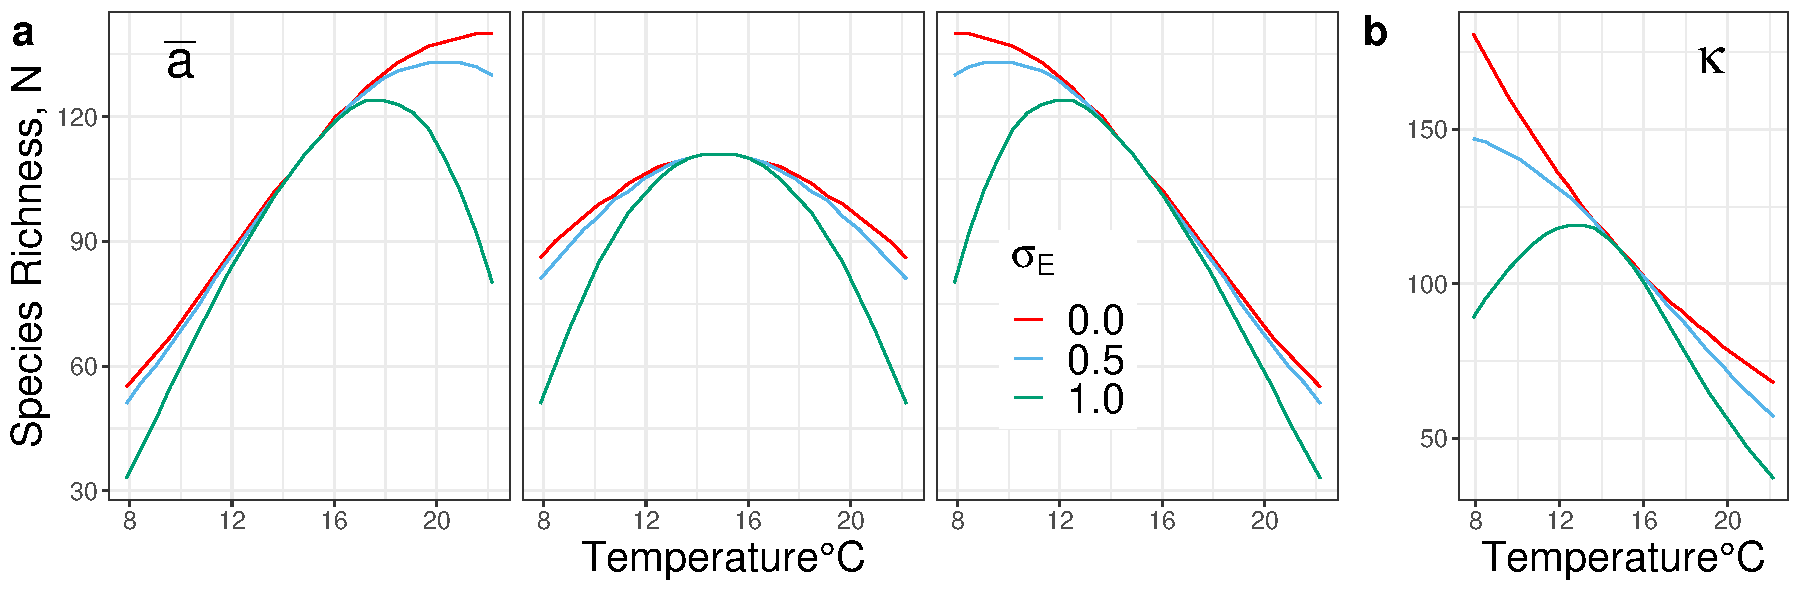
\includegraphics[width=0.8\textwidth]{docs/Figures/Fig_N_ana.pdf} 
    \caption{\textbf{The thermal response of species richness  varies with the distribution of thermal sensitives} a) The shape of distribution of thermal sensitivities of interactions $E_a$ alters the richness-temperature relationship. As predicted by \cref{EQ:Boltz_dist} the average thermal sensitivity (as shown in each panel) determines the overall direction of the thermal response whilst variance in thermal sensitivity (coloured lines, see legend) introduces additional curvature to the species richness response. b) Altering the variation in the thermal sensitivity of $\kappa$ has the same effect, creating curvature in  the species richness response (colored lines). Curves were generated using the approach outlined in methods with parameters $\sigma{\log(K_0)} = 0.5$, $\sigma_{E_K} = 0.2$, $\mu_{a_0} = log(0.01)$ and  $\sigma_{a_0} = 0.5$}
    \label{Fig:N_vs_T}
\end{figure}


\subsection*{Empirical variation in thermal sensitivity is relevant for community level thermal responses}

Our empirical dataset on the thermal performance of microbial growth showed significant variation in the thermal sensitivity of $K$ (\cref{Fig:TPC_data}). Normal distribution fits using maximum likelihood estimation yielded estimates of $\log(K_0) \sim \mathcal{N}(-0.14,0.58)$ and $E_K \sim \mathcal{N}(0.06,0.29)$ for the normalisation constant and sensitivity respectively (\cref{Fig:TPC_data}a-b). As expected, this empirically observed variation in the thermal sensitivity resulted in a unimodal response of species richness to temperature whilst the no-variation scenario resulted in a simple monotonic response (\cref{Fig:TPC_data}c). 

\begin{figure}[H]
    \centering
    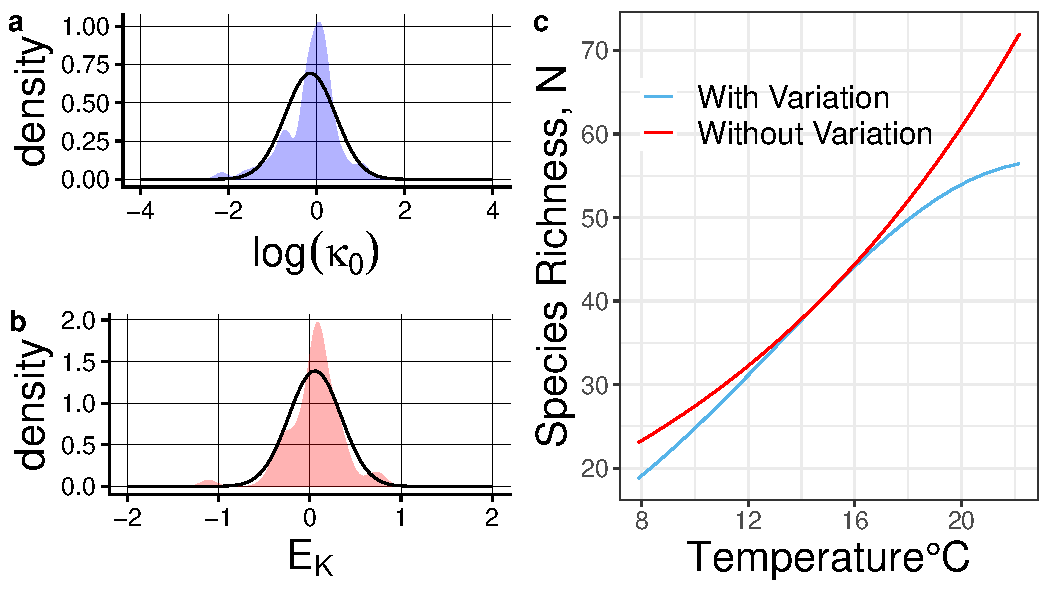
\includegraphics[width = 0.8\textwidth]{docs/Figures/MTE_fig.pdf}
    \caption{\textbf{Empirical levels of variation in thermal sensitivity alters the thermal response of species richness }. a-b) Distributions of empirical estimates of a) $\log(K_0)$ and b) $E_K$. Colored density plots are the actual empirical distributions of the parameters with the solid black line showing the fitted normal distribution. The distribution of thermal sensitivity (b) demonstrates the existence of variation in the thermal response ($\sigma_{E_K} = 0.29$. c) Prediction of species richness thermal response using the empirical distributions. The blue and red lines represent the estimates with and without variance in thermal sensitivity, showing how the observed variance creates a unimodal response of species richness to temperature.}
    \label{Fig:TPC_data}
\end{figure}

\subsection*{The distribution of thermal sensitivities predicts the species richness of randomly assembled communities}

Overall the relationship between temperature and species richness in community assembly simulations followed the same expected qualitative patterns across all three interaction scenarios, taking an increasingly unimodal shape as variation in thermal sensitivity $\sigma_E$ increased (\cref{Fig:Temperature_assembly,Fig:Temperature_assembly_mixed}). The actual thermal response of species richness was predicted well by the analytical expression in the competitive scenario (where $a_{ij} > 0$) with the predictions for species richness falling within the ranges observed in the numerical simulations (\cref{Fig:Temperature_assembly}b). This pattern was consistent across the different levels of variation in thermal sensitivity though they tended to overestimated the decline in richness at higher temperatures at the highest level of variation (\cref{Fig:Temperature_assembly}c). In the two mixed interaction scenarios the qualitative patterns in the thermal response (i.e., the increase in unimodality and general direction) followed the analytical expectations (\cref{Fig:Temperature_assembly_mixed}). This result is verified by the increase in the absolute size in the quadratic coefficient with increasing variation in thermal sensitivity (\cref{SIFig:quad_coeff}).

\begin{figure}[H]
    \centering
    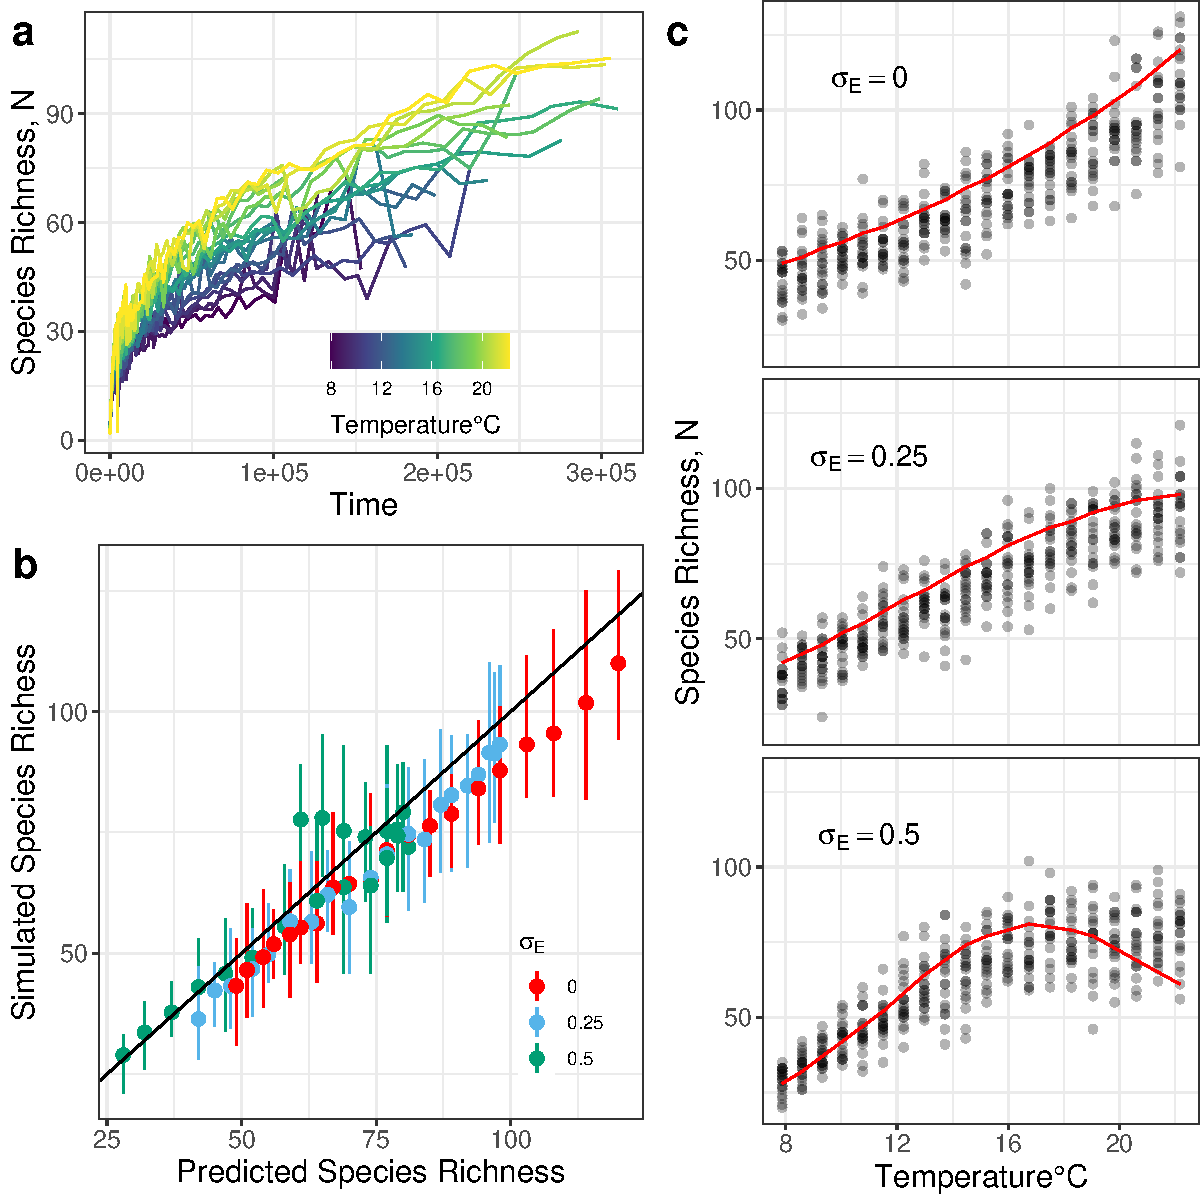
\includegraphics[width = 0.8\textwidth]{docs/Figures/Fig_sim.pdf}
    \caption{\textbf{The assembly of ecosystems at different temperatures is predicted by the analytical feasibility condition} A) Trajectories of species richness over assembly across temperature at a single level of variation in $E$ ($\sigma_a = 0.25$). Each line is the average species richness over time at a given temperature across 20 replicates. B) The final species richness reached by the assembly simulations plotted against the analytical predictions. Each point is the average species richness across the 20 replicates with error bars showing the 5\% and $95$\% percentiles. The black line represents the 1:1 line where predictions match the simulations. C) The species richness - temperature relationship at 3 levels of variation in $E$. Each points represents the species richness reached by a single assembly simulation with the red line representing the predicted species richness at a threshold of $0.001$. Overall the observed species richness and predictions match well with most observations.}
    \label{Fig:Temperature_assembly}
\end{figure}

\begin{figure}
    \centering
    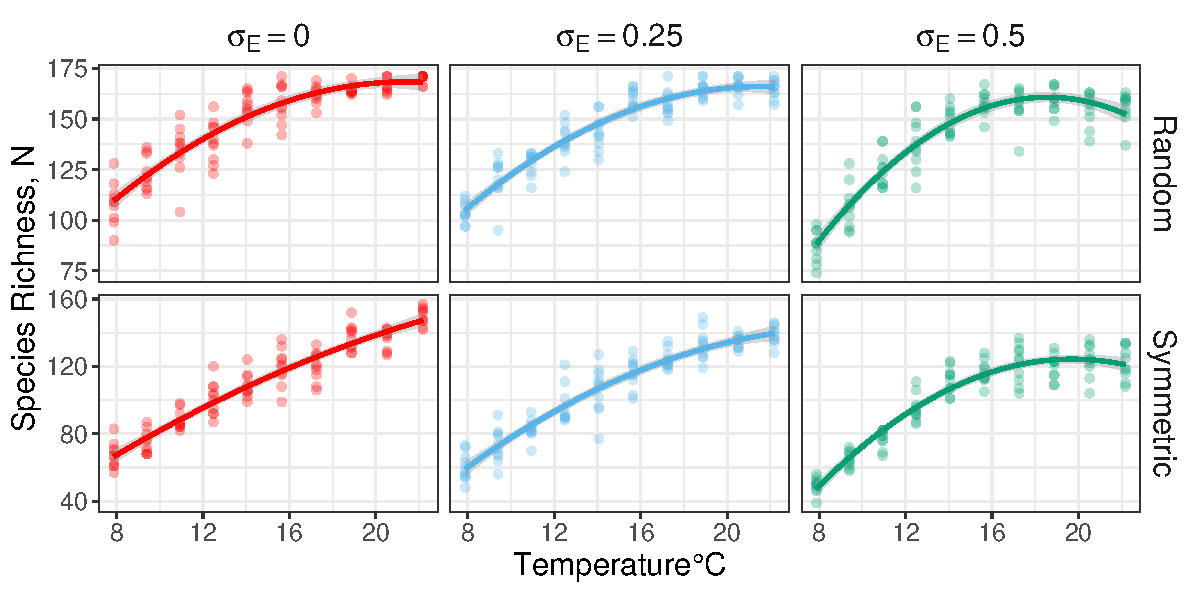
\includegraphics[width = 0.8\textwidth]{docs/Figures/Fig_mixed.pdf}
    \caption{\textbf{Variation in thermal sensitivity alters the richness-temperature relationship with mixed interaction types} The qualitative pattern predicted by the analytical results, that increased variation will lead to increased unimodality in the thermal response of richness, holds across the two mixed interaction scenarios. Each point represents the final richness reached by a single assembly simulation with the line representing a quadratic polynomial fit to aid in visualisation  of the increase in unimodality. Panels show increasing values of $\sigma_E$ moving left to right and the random and symmetric interactions case above and below.}
    \label{Fig:Temperature_assembly_mixed}
\end{figure}

\newpage

\section*{Discussion}
We have investigated how variation in population-level thermal responses affects the temperature dependence of species richness in microbial communities, deriving new analytical results which explicitly link this variation to emergent community dynamics which constrain maximal species richness. We further support this new mechanism lining variation in thermal responses to species richness with analysis of a new data set on microbial population growth and numerical simulations. This represents the first attempt to understand this population-level variation and how it scales up to affect the thermal responses at the community level. 

One of the core insights from our analytical results is that increased variation in thermal sensitivity $\sigma_E$ results in unimodality in the microbial richness-temperature curve, a pattern that emerges due to the exponential nature of individual thermal responses. This result provides a new mechanism through which temperature may act to influence microbial community richness which we expect will partially drive patterns of microbial richness in nature in conjunction with other previously suggested mechanisms such as the metabolic niche hypothesis (REF) and the metabolic theory of biodiversity (REF) discussed above. We expect the mechanism we suggest here will be relevant in real systems because of: 1) the documented widespread variation in thermal sensitivities that exists across microbial taxa both in previous work (REF) and in our analysis of microbial population growth curves here, and 2) the results of our simulations of community assembly which suggest that the general insight that variation leads to unimodality holds over a range of structures of interspecies interactions . 

In demonstrating the importance of this variation in thermal sensitivity our results align with recent work looking at variation in thermal responses. In terms of data, our analysis of a newly compiled data set of microbial growth curves demonstrates significant variance in thermal sensitivity, a result that is in agreement with the large body of literature documenting the existence of this variation both between microbial taxa (REF) and across the tree of life more generally (REF). Interestingly our estimates of the thermal sensitivity of carrying capacity $K$ centered very close to zero, suggesting that, at least in our data set, there is no bias in the direction of it's thermal response. This is in contrast to previous theoretical work predicting that the thermal sensitivity of $K$ should follow the inverse of metabolic rate (REF) which for microbes has a $E$ value of $\approx 0.9$ (REF)(which would predict $\mu_{E_K} \approx -0.9$).

In addition to quantifying the amount of variation in thermal sensitivity our results also agree with previous work demonstrating the importance of this variation in driving ecological dynamics and their responses to temperature. Previous studies trying to understand the effects of this variation have tended to use simple ecological models consisting of a small numbers of interacting populations, allowing explicit consideration of the differences in $E$ values between individual populations (REF). Our results agree with the general principle that this variation is important but crucially extends this approach to a more general model of complex multi-species communities. This represents the first attempt to consider the effects of variation in thermal responses across populations on emergent community properties, representing a significant advance in our understanding of the scaling up of population-level responses to the community level. We note here that whilst we focus on species richness in microbial communities, we expect that the approach we use to should be generally applicable to other properties of interest, such as ecosystem functioning, and other types of ecological systems beyond microbial communities. 

The general applicability of our results is supported by the our community assembly simulations which show that our insights into the effect of variation on the thermal response of species richness hold under a range of interspecies interaction structures. Under the two mixed interaction scenarios we observed the predicted increase in unimodality in the temperature-richness relationship with increasing variation in $E$. This can be explained by the fact that the mechanism driving the unimodal relationship (i.e., the variation  in thermal sensitivity being passed through the exponential like thermal response in \cref{EQ:Boltz_dist}) is still present despite the fact that these scenarios represent deviations from the requirements of the feasibility condition, preventing us from bounding species richness and predicting its thermal response explicitly. This result poses an interesting question of how general our insight here is and suggests that it may predict qualitative patterns in richness across other model structures. One particularly interesting test specific to microbial communities would be to consider the modified MacArthur consumer-resource model which has recently found popularity as a way model the microbial communities dominated by metabolite-exchange mediated interactions (REF). Previous work has demonstrated that these models can exhibit vary different dynamics to the GLV due to the fact that interactions are not modeled directly but rather through the consumption and production of shared resource pools (REF). Thus, it is unclear whether our general result regarding variation would apply or whether the complex non-linear interactions dynamics would cloud such patterns emerging. 

In addition to considering other model structures one logical extension of our work would be to consider community dynamic properties beyond feasibility, which we use here as a means to constrain species richness. As discussed previously feasibility is the most basic requirement for the persistence of a community through time, ensuring simply that a fixed point exists at which all species' biomass are greater than zero (REF). Feasibility does not tell us about how this fixed point responds to perturbations and will not tell us when an equilibrium is unstable, which will ultimately determine its ability to persist (REF). By using other measures of community dynamics such as local stability (The capacity of system to return to equilibrium following a small perturbation; REF) or reactivity (The rate at which a system returns to equilibrium following perturbation; REF) one would be able to further constrain the number of populations a given communities can support, thus improving our understanding of the temperature response of species richness. 

In conclusion we have derived new analytical results which explicitly link the variation in the thermal responses between microbes to emergent community dynamics and their species richness. We show with a meta-analysis that such variation both exists and is sufficient to alter predictions of the species richness over thermal gradients and that the insights afforded by our analytical work are robust and apply over a range of interaction structures.

\newpage

\bibliography{Temp_richness.bib}

\section*{Supplementary Material}

\paragraph{Supplementary Material section 1} \textbf{Mean-field approximation}

\paragraph{Supplementary Material section 2} \textbf{Derivation of thermal response distributions}

\paragraph{Supplementary Figure 1} \textbf{Quadratic Coefficients for mixed interaction assembly simulations}


\end{document}